\begin{figure}[H]
\centering
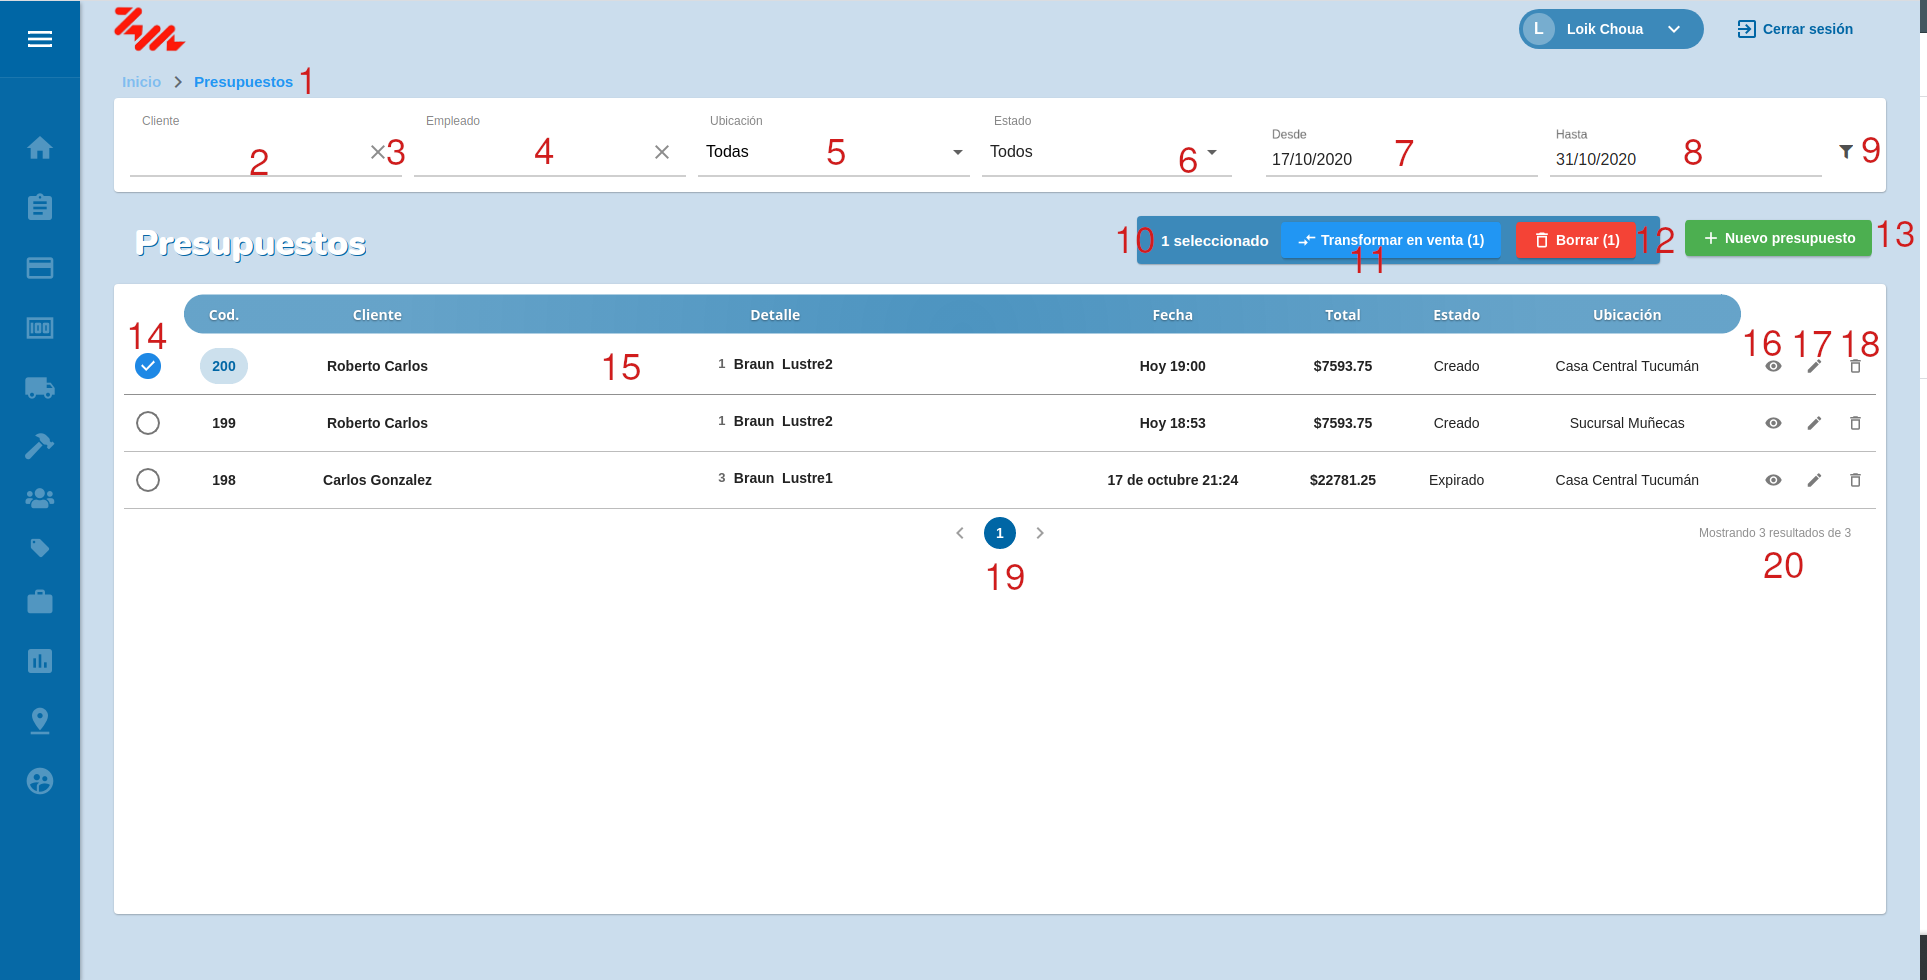
\includegraphics[width=\textwidth,height=\textheight,keepaspectratio]{Escenarios/AD-03-00}
\caption{Escenario - AD-03-00}
\label{fig:AD-03-00}
\end{figure}
Este escenario muestra toda la información referida a los presupuestos, junto con las acciones disponibles.
El botón \textbf{AD-03-01} permite navegar al escenario \textbf{AD-02-00}. El campo \textbf{AD-03-02} permite ingresar un cliente para filtrar los presupuestos por cliente, el campo cuenta con el botón \textbf{AD-03-03} que permite borrar el texto ingresado en el campo. El campo \textbf{AD-03-04} permite al usuario buscar presupuestos de acuerdo al empleado que lo realizó. La lista desplegable \textbf{AD-03-05} permite filtrar de acuerdo a la ubicación en dónde se creó el presupuesto. La lista desplegable \textbf{AD-03-06} permite al usuario filtrar por los estados en los cuales puede encontrarse el presupuesto. Los campos  \textbf{AD-03-07} y \textbf{AD-03-08} permiten al usuario filtrar los presupuestos de acuerdo a un rango de fechas en la cual fueron creados. El botón \textbf{AD-03-09} permite visualizar más filtros de búsqueda disponibles, como ser el producto, la tela y el lustre.
El campo \textbf{AD-03-10} se muestra cuando se ha seleccionado al menos un presupuesto de la tabla, e indica la cantidad de presupuestos seleccionados. El botón \textbf{AD-03-11} permite al usuario crear una venta a partir de uno o más presupuestos seleccionados y navega al escenario \textbf{AD-08-00}. El botón \textbf{AD-03-12} permite borrar los presupuestos que fueron seleccionados. El botón \textbf{AD-03-13} permite al usuario crear un nuevo presupuesto y navega al escenario \textbf{AD-04-00}.
El botón \textbf{AD-03-14} permite al usuario seleccionar uno o más presupuestos del resultado de la búsqueda. El campo \textbf{AD-03-15} muestra la información relacionada a los presupuestos especificando el código, el cliente para el cual se le realizó, el detalle de presupuesto, la fecha de creación, el total del presupuesto, el estado en el cual se encuentra y la ubicación en el cual fue creado. El botón \textbf{AD-03-16} permite navegar al escenario \textbf{AD-06-00} para ver el presupuesto, el botón \textbf{AD-03-17} permite al usuario editar el presupuesto navegando al escenario \textbf{AD-04-00} y el botón \textbf{AD-03-18} permite al usuario borrar el presupuesto. 
En  \textbf{AD-03-19} se mostrarán las páginas de resultado, pudiendo cambiar de página. En \textbf{AD-03-20} se mostrará cuantos resultados se están visualizando y el total.
\clearpage
